\documentclass[twocolumn, 11pt]{article}%
\usepackage{amsmath, amssymb, esint, gensymb, hyperref}
\usepackage{graphicx, cuted, geometry, float, scalerel, xcolor, chemfig}
\newcommand\sbullet[1][.5]{\mathbin{\ThisStyle{\vcenter{\hbox{%
  \scalebox{#1}{$\SavedStyle\bullet$}}}}}%
}

\geometry{
    a4paper,
    total={170mm,260mm},
}

\begin{document}

\begin{strip}
  \vspace*{\dimexpr-\stripsep}
  \begin{center}
      \Large\textbf{FISIKA 2}\\
      \large{Pertemuan 1 - Minggu 3 (233161)}\\
      \large{\today}
   \end{center}
\end{strip}

\section{Hukum Gauss}
    \subsection{Fluks Listrik}%
    \begin{center}
        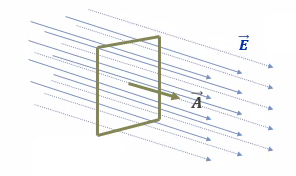
\includegraphics[width=100px]{1.png}
    \end{center}
    Didefinisikan sebagai $\Phi$ pada medan listrik melalui permukaan A,
    \[\Phi = \vec E \sbullet[.75] \vec A \]
    atau bisa juga ditulis (karena perkalian dot hasilnya adalah skalar)
    \[ \Phi = E\ A \cos \theta \]

    Dimana $\vec A$ adalah vektor normal ke permukaan (besar A, dan arah normal ke permukaan). Lalu $\theta$ adalah  adalah sudut antara $\vec E$ dan $\vec A$

    \begin{center}
        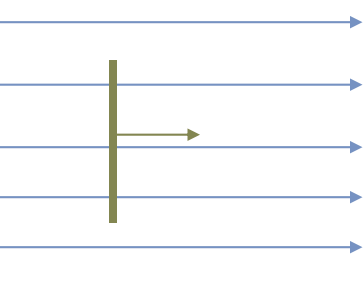
\includegraphics[width=100px]{2.png}
    \end{center}

    Fluks dapat dianggap sebagai jumlah garis medan yang menembus suatu permukaan. Fluks bergantung pada besar medan listrik, luas permukaan, dan orientasi relatif antara medan dan permukaan. Fluks juga bergantung dengan orientasi penampang luas (semakin besar $\theta$ semakin kecil $\cos \theta$, maks $\frac{\pi}{2}$ rad).
    \begin{center}
        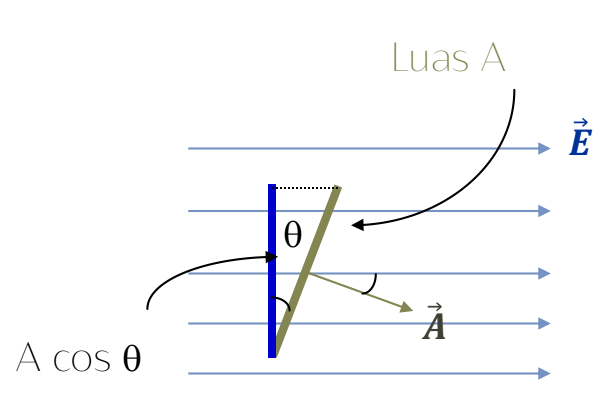
\includegraphics[width=100px]{3.png}
        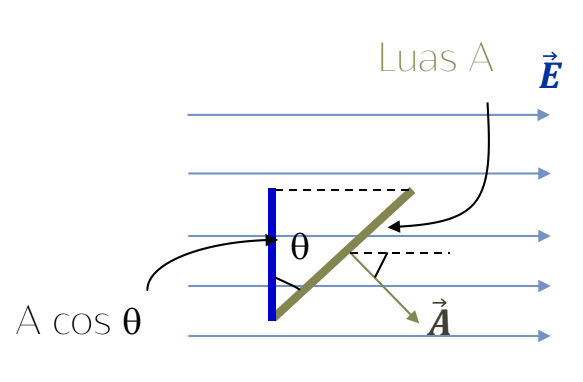
\includegraphics[width=100px]{4.png}
    \end{center}

    \subsection{Fluks Listrik Permukaan Melengkung Atau Bidang Bervariasi Terhadap Posisinya}%
    
    \begin{center}
        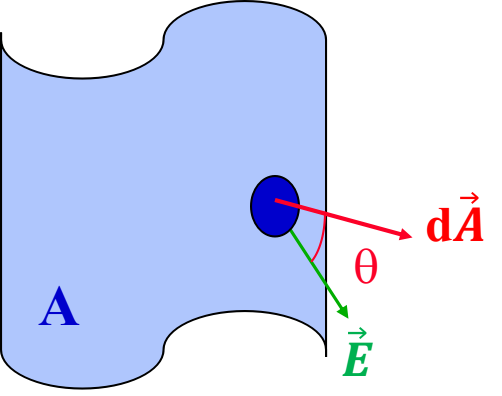
\includegraphics[width=100px]{5.png}
    \end{center}

    \begin{itemize}
        \item Kita perlu membagi permukaan menjadi daerah kecil dengan luas $dA$
        \item Fluks melalui $dA$ adalah :
            \[ d \Phi= E\ dA \cos \theta \]
            \[ d \Phi= \vec E\ \sbullet[.75] d \vec A \]
        \item Untuk mendapatkan fluks total, kita perlu mengintegralkan permukaan $A$
            \[ \Phi = \iint d\theta = \iint \vec E \sbullet[.75] d \vec A\]
    \end{itemize}

    \subsection{Dalam Kasus Permukaan Tertutup}%

    \begin{center}
        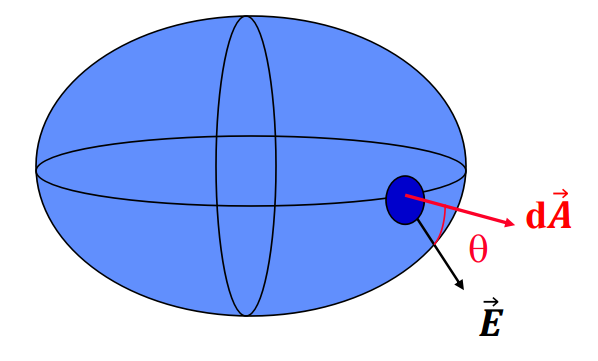
\includegraphics[width=150px]{6.png}
    \end{center}
    
    \[ \Phi = \oiint d \Phi = \oiint \vec E \sbullet[.75] d \vec A \]
    Tanda lingkaran pada integral dobel berarti integral atas permukaan dua dimensi yang tertutup.\\

    Untuk permukaan tertutup, \textbf{fluks positif} untuk garis-garis medan yang keluar dari volume tertutup. \textbf{Fluks negatif} untuk garis-garis medan yang masuk ke permukaan tertutup.

    \begin{center}
        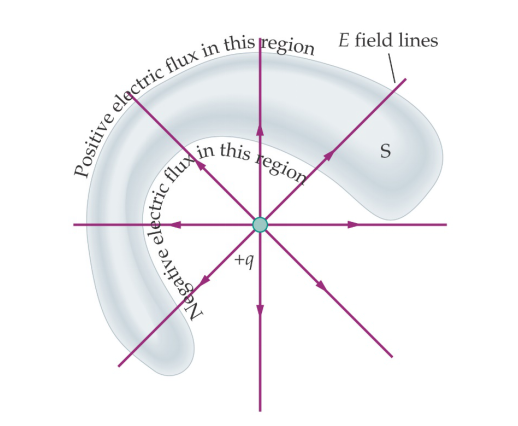
\includegraphics[width=150px]{7.png}
    \end{center}

    Jika \textbf{muatan berada di luar permukaan tertutup, fluks netto sama dengan nol}. Banyaknya garis medan yang meninggalkan permukaan sama dengan yang memasukinya.

    \section{Permukaan Bola Dengan Muatan Titik Di Tengah}%

    \begin{center}
        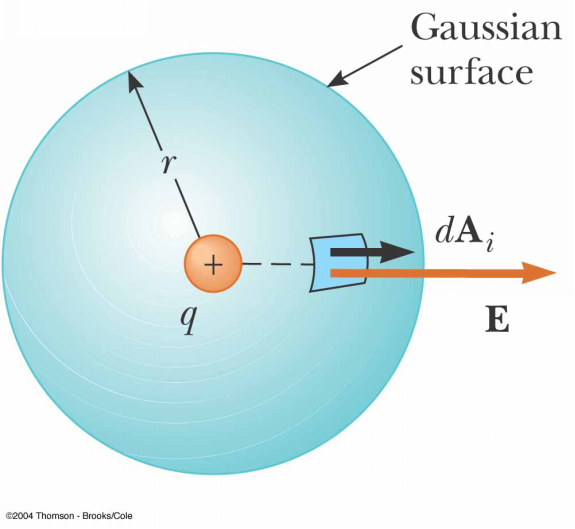
\includegraphics[width=150px]{8.png}
    \end{center}

    Fluks medan listriknya ialah..
    \begin{align*}
        \Phi = \oiint d \Phi &= \oiint \vec E \sbullet[.75] \vec A\\
        \Phi &= \oiint E\ dA \cos \theta\\
             &= \oiint \frac1{4\pi \epsilon_0} \frac{q\ dA}{r^2}
    \end{align*}

    Dengan $\displaystyle \frac{dA}{r^2}=d\Omega$, maka

    \begin{align*}
        \Phi &= \frac{q}{4\pi \epsilon_0} \oiint d\Omega\\
             &= \frac{q}{4\pi \epsilon_0} 4\pi\\
             &= \frac{q}{\epsilon_0}
    \end{align*}
    
    Inilah yang dinamakan dengan Hukum Gauss, dimana Fluks listrik yang melalui permukaan tertutup sama dengan $\sum$ (jumlah) muatan tertutup dibagi dengan $\epsilon_0$
    
    \subsection{Hukum Gauss}%
    
    \[ \oiint \vec E \sbullet[.75] d \vec A = \frac{q_{enclosed}}{\epsilon_0} \]

    Atau jika terdapat banyak muatan
    
    \[ \oiint \vec E \sbullet[.75] d \vec A = \frac{\sum\limits_{inside}q}{\epsilon_0} \]

    Medan listrik dapat dengan mudah ditentukan dengan menerapkan Hukum Gauss (khusus untuk kasus sistem yang sangat simetris). Seperti contoh berikut

    \begin{center}
        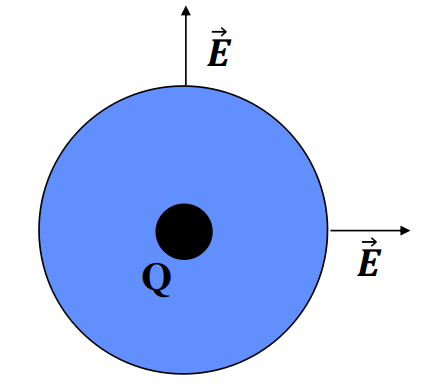
\includegraphics[width=100px]{10.png}
    \end{center}

    \begin{align*}
        \oiint \vec E \sbullet[.75] d\vec A &= \frac{q}{\epsilon_0}\\
                                &= E \oiint dA\\
                                &= E\ A\\
    \end{align*}
    
     Jika diketahui $A=4\pi r^2$, maka

    \begin{align*}
        E\ A &=E\ 4\pi r^2\\
             &= \frac{q}{\epsilon_0}\\
             &= \frac1{4\pi \epsilon_0} \frac{q}{r^2}
    \end{align*}
    
    Dimana
    \[ k=\frac1{4\pi \epsilon_0} \]
    $\epsilon_0$ adalah permitivitas ruang hampa yang nilainya $8.85 \times 10^9\ C^2/Nm^2$. Bisa dibuktikan bukan, itu adalah Hukum Coulomb.

    \subsection{Penerapan Hukum Gauss}%

    Hukum Gauss hanya berguna saat medan listrik konstan pada permukaan tertentu.

    \begin{figure}[h!]
        \centering
        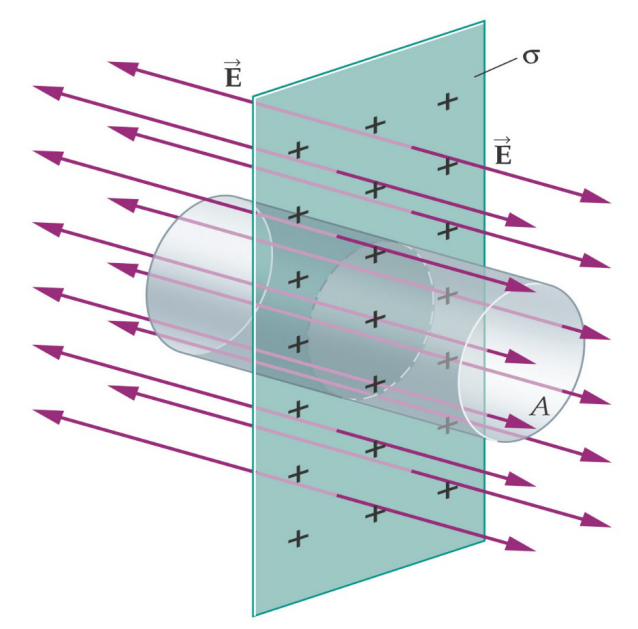
\includegraphics[width=100px]{11.png}\\
        Lembar muatan yang tak terbatas
    \end{figure}

    \begin{enumerate}
        \item Pilih Permukaan Gauss, dalam hal ini berbentuk pil silinder.
        \item Hitung fluks dari medan listrik melalui Permukaan Gauss
            \[ \Phi = 2EA \]
        \item Persamaan
            \[ \Phi = \frac{q_{enclosed}}{\epsilon_0} \]
            \[ 2EA=\frac{q_{enclosed}}{\epsilon_0} \]
        \item Selesaikan pada E
            \[ E=\frac{q_{enclosed}}{2A\epsilon_0}=\frac{\sigma}{2} \]
            dengan $\displaystyle\sigma=\frac{q_{enclosed}}{A}$
    \end{enumerate}

    \subsection{Hukum Gauss-Simetri Khusus}%
    \begin{center}
        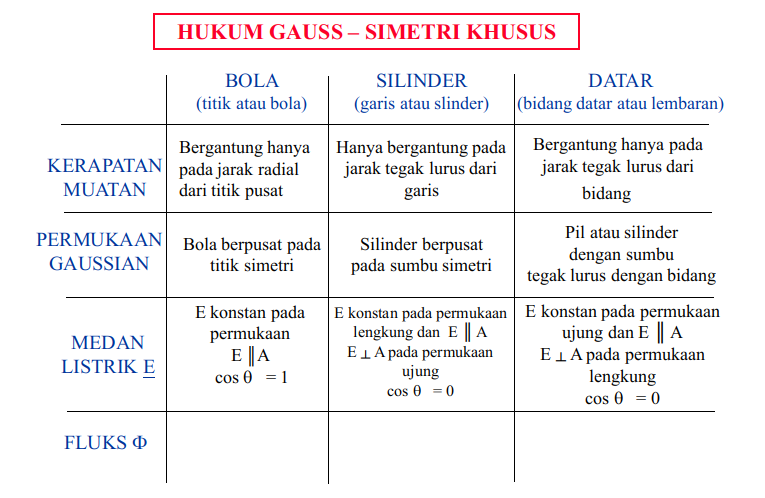
\includegraphics[width=220px]{12.png}
    \end{center}

    \begin{center}
        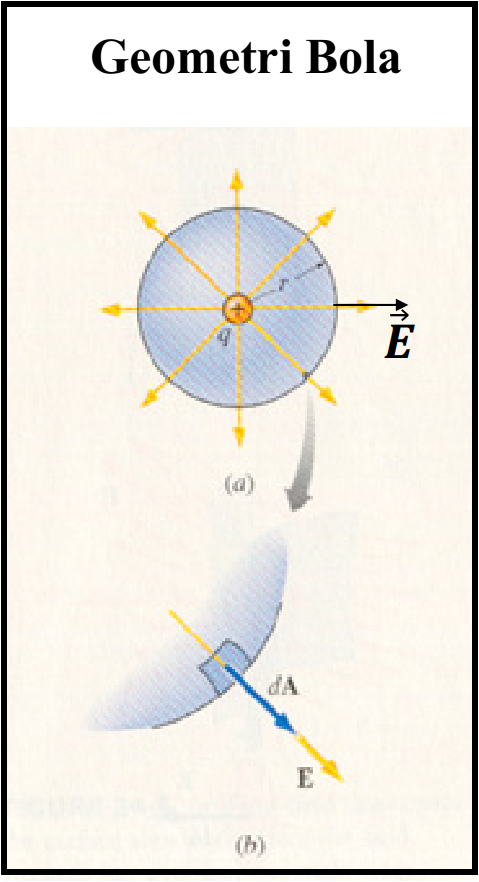
\includegraphics[width=80px]{13.png}
        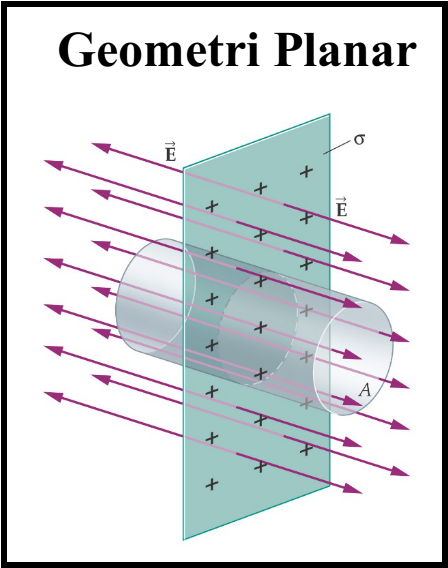
\includegraphics[width=80px]{14.png}
        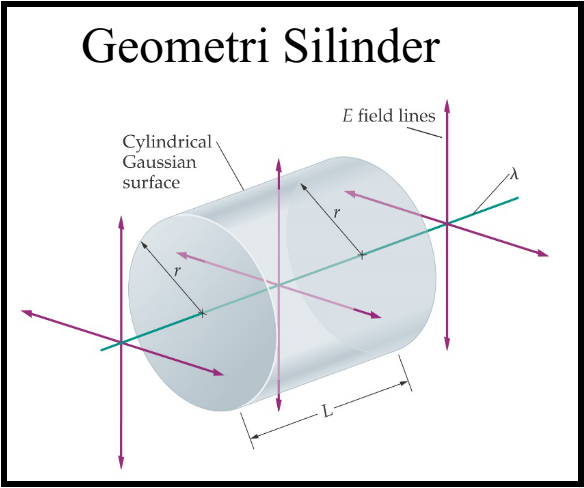
\includegraphics[width=80px]{15.png}
    \end{center}

    \section{Implikasi Hukum Gauss Untuk Konduktor}%
    \begin{itemize}
        \item Untuk konduktor bermuatan, dalam situasi statis, semua muatan berada di permukaan konduktor.
        \item Untuk konduktor bermuatan, dalam situasi statis, medan listrik adalah nol di dalam seluruh konduktor, dan tegak lurus dengan permukaan di luar.
    \end{itemize}

    Perlu diketahui bahwa $\vec E = 0$ di dalam sebuah konduktor, mengapa? Konduktor penuh dengan elektron bebas, kira-kira satu per kubik Angstrom. Jika $\vec E$ bukan nol di beberapa  daerah, maka elektron yang berada di sana merasakan sebuah kekuatan $-e\vec E$ dan mulai bergerak.

    Dalam soal elektrostatika, elektron bergerak menyesuaikan posisi sampai gaya pada setiap elektron adalah nol (atau kalau tidak, elektron akan tetap bergerak). Itu artinya saat kesetimbangan tercapai, $\vec E =0$ pada seluruh bagian dalam konduktor.

    Oleh karena $E=0$ di dalam konduktor, maka bagian dalam konduktor adalah netral.

    \begin{center}
        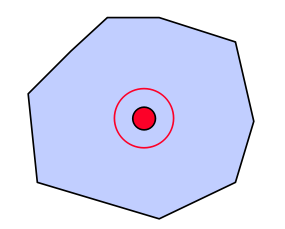
\includegraphics[width=100px]{16.png}
    \end{center}

    Misalkan terdapat muatan tambahan $\color{red}\bullet$ di dalam. Hukum Gauss untuk permukaan bola kecil mengatakan akan ada E yang tidak bernilai nol di dekatnya. Tapi tidak mungkin ada, di dalam sebuah logam!

    \begin{center}
        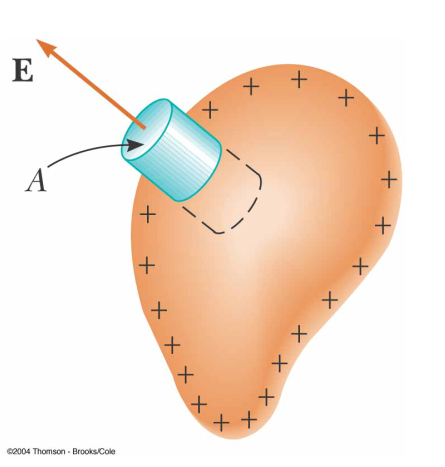
\includegraphics[width=100px]{17.png}
    \end{center}

    \textcolor{red}{Akibatnya bagian dalam logam menjadi netral. Setiap kelebihan muatan akan berakhir di permukaan logam.}

    \subsection{Sifat Konduktor}%
    Dalam sebuah konduktor ada banyak elektron yang bebas bergerak. Fakta ini memiliki beberapa konsekuensi yang menarik.

    \begin{itemize}
        \item Kelebihan muatan yang ada pada sebuah konduktor, akan bergerak keluar permukaan konduktor.\\
            \begin{center}
                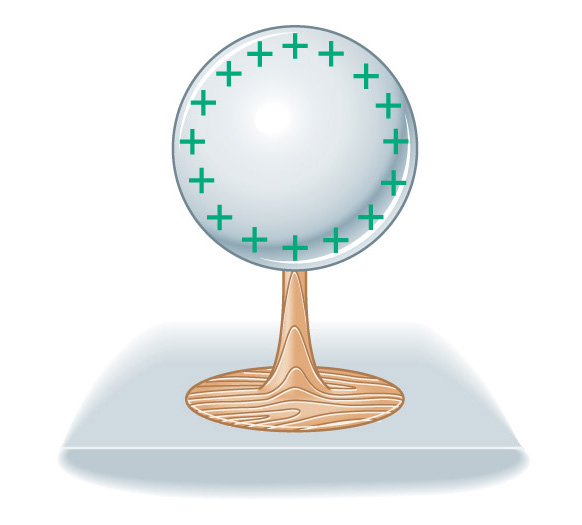
\includegraphics[width=100px]{18.png}
            \end{center}
        \item Medan listrik di dalam konduktor bernilai 0 saat diisi dalam kondisi tidak terpakai.
        \item Konduktor melindungi rongga di dalamnya dari medan listrik eksternal.
        \item Garis-garis medan listrik menghubungkan permukaan konduktor pada sudut yang tepat.
            \begin{center}
                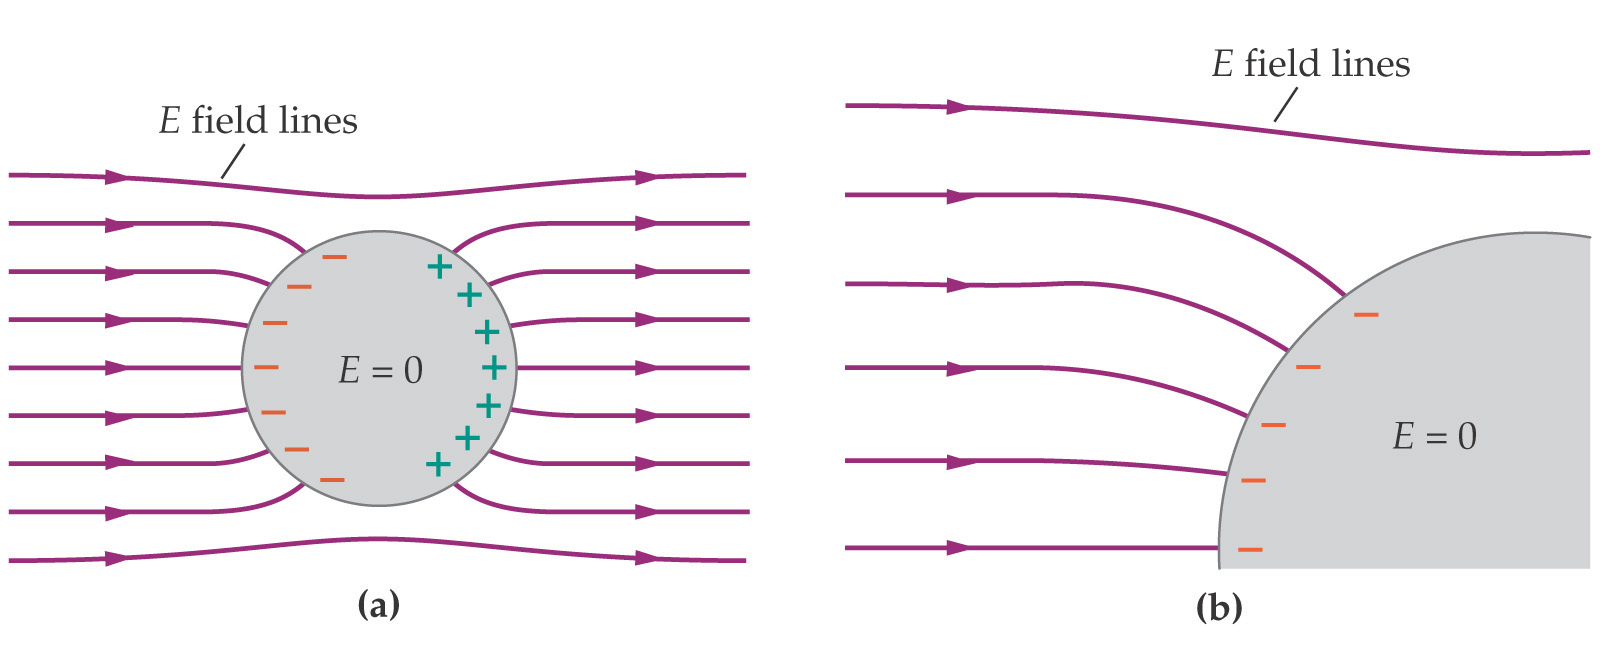
\includegraphics[width=200px]{19.png}
            \end{center}
        \item Konduktor dapat dimuati melalui kontak atau induksi.
            \begin{center}
                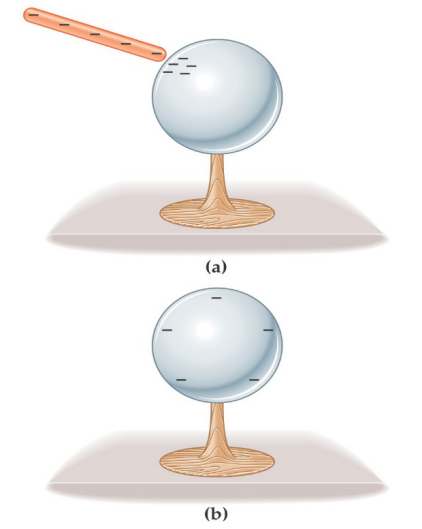
\includegraphics[width=100px]{20.png}
                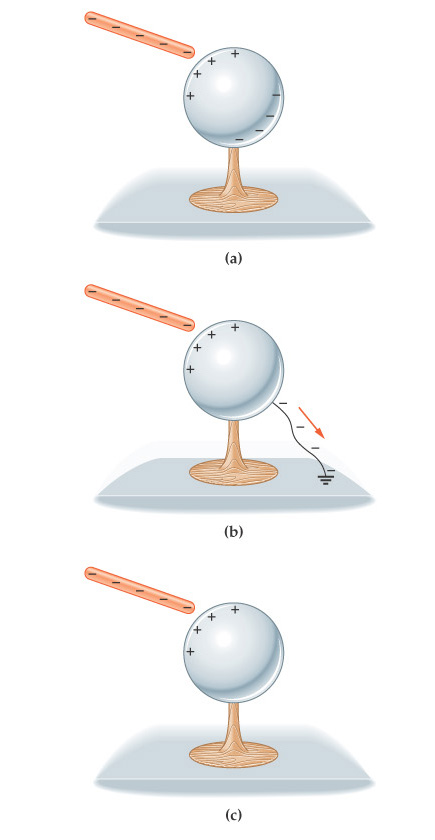
\includegraphics[width=100px]{21.png}
            \end{center}
        \item Menghubungkan sebuah konduktor pada tanah disebut dengan grounding. Tanah dapat menerima elektron dalam jumlah yang tidak terbatas.
    \end{itemize}
    
    \subsection{Problem : Kabel Koaksial Terisi muatan}%
    Gambar ini adalah penampang garis muatan yang sangat panjang, dikelilingi oleh konduktor silinder yang panjangnya tak terhingga.  Temukan $\vec E$.

    \begin{center}
        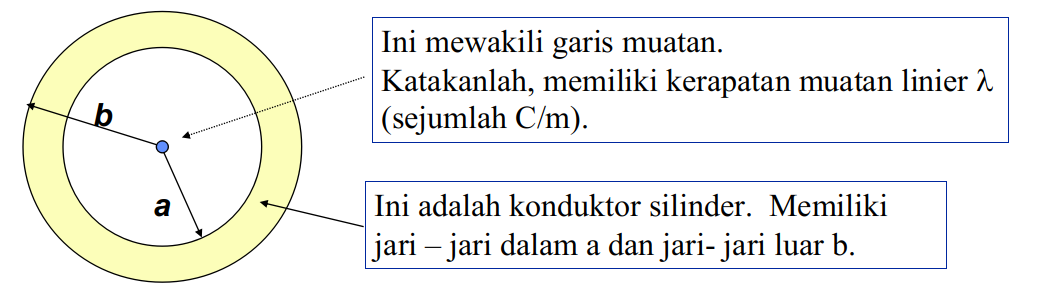
\includegraphics[width=200px]{22.png}
    \end{center}

    \textcolor{red}{\textbf{GUNAKANLAH SIMETRI!}}

    Jelas $\vec E$ mengarah ke luar, dan amplitudonya hanya bergantung pada $r$.

    Pertama, temukan $E$ pada posisi dalam ruang di dalam silinder $(r<a)$.
    \begin{center}
        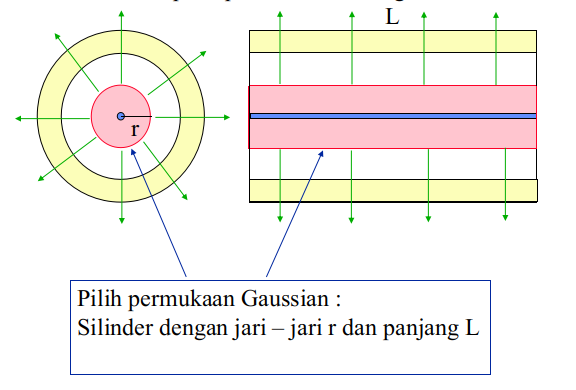
\includegraphics[width=200px]{23.png}
    \end{center}

    \begin{enumerate}
        \item Berapa muatan yang dilingkupi? $\Rightarrow \lambda L$.
        \item Berapakah fluks yang melewati tutup ujung? $\Rightarrow \cos 90\degree=0$.
        \item Berapakah fluks yang melewati permukaan lengkung? $\Rightarrow EA = E(2\pi rL)$.
        \item Total Fluks = $E(2\pi rL)$.
        \item Hukum Gauss $\Rightarrow E(2\pi rL)=\frac{\lambda L}{\epsilon_0}$, jadi
            \[ E(r)=\frac{\lambda}{2\pi r\epsilon_0} \]
    \end{enumerate}

    Sekarang cari $E$ pada posisi di dalam silinder $(a<r<b)$.\textcolor{blue}{Tidak ada medan listrik dalam konduktor $\vec E=0$}.

    Tetap saja kita bisa bisa belajar sesuatu dari hukum Gauss.

    Buat silinder Permukaan Gaussian jenis yang sama. Sekarang sisi yang melengkung seluruhnya di dalam konduktor, di mana $\vec E=0$; karenanya fluksnya adalah nol.

    \begin{center}
        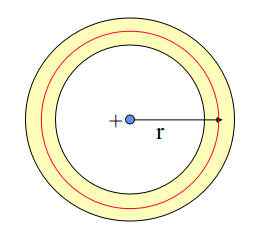
\includegraphics[width=130px]{24.png}
    \end{center}

    \textcolor{red}{Jadi total muatan tertutupnya oleh permukaan seperti ini harus nol.}

    Harus ada muatan per satuan panjang $-\lambda$ yang tertarik ke permukaan bagian dalam logam sehingga muatan total yang tertutup oleh permukaan Gaussian ini adalah nol.

    \begin{center}
        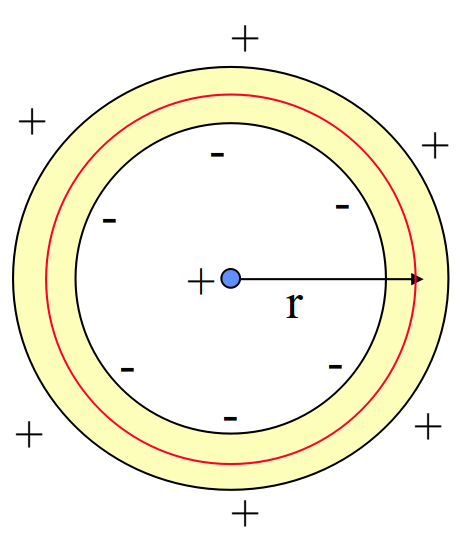
\includegraphics[width=130px]{25.png}
    \end{center}

    Dan karena silindernya netral, muatan negatif pasti datang dari luar permukaan. Jadi permukaan luarnya memiliki kerapatan muatan per satuan panjang $+\lambda$ yang tersebar di sekeliling permukaan luar.

\section{Implikasi Hukum Gauss Untuk Isolator}%
    \subsection{Problem: Bola Isolator Bermuatan Q}%

    \begin{center}
        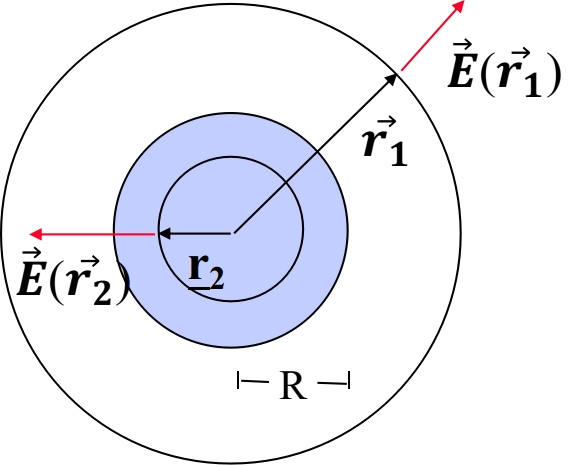
\includegraphics[width=130px]{26.png}
    \end{center}

    Muatan $Q$ didistribusikan secara seragam melalui bola berjari-jari $R$. Bagaimana medan listriknya sebagai fungsi dari $\vec r$?\\
    Tentukan $\vec E$ pada $\vec r_1$ dan $\vec r_2$.\\

    \textcolor{red}{\textbf{GUNAKANLAH SIMETRI!}}\\

    Ini adalah bola yang simetris. Artinya $\vec E (\ \vec r\ )$ secara radial keluar, dan semua menunjuk pada radius yang diberikan $(\mid \vec r\mid=r)$, dan memiliki besar bidang yang sama.\\

    Pertama, temukan $\vec E (\ \vec r\ )$ pada titik di luar bola bermuatan. Gunakanlah Hukum Gauss, menggunakan Permukaan Gaussian pada bola yang berjari-jari $r$ seperti yang dapat dilihat pada gambar.

    \begin{center}
        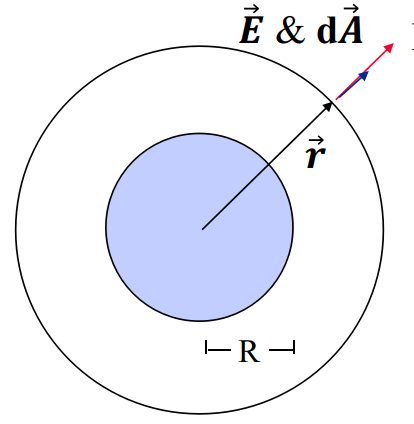
\includegraphics[width=130px]{27.png}
    \end{center}

    \textcolor{blue}{Sama seperti medan listrik oleh muatan titik! (untuk $r>R$)}

    Berapa muatan yang terlingkupi? $\Rightarrow Q$\\
    Berapakah fluks yang melalui permukaan ini?

    \begin{align*}
        \Phi &= \oiint \vec E \sbullet d\vec A\\
             &= \oiint E\ dA\\
             &= E \oiint dA\\
             &= EA\\
             &= E(4\pi r^2)
    \end{align*}

    Menurut Gauss
    \[ \Phi = \frac{Q}{\epsilon_0} \]

    Jadi
    \[ \vec E (\vec r\ ) = \frac1{4\pi r^2} \frac{Q}{r^2} \hat r \]\\

    Selanjutnya kita harus menentukan $\vec E (\vec r\ )$ pada titik \textbf{di dalam} bola. Terapkan Hukum Gauss, menggunakan bola kecil berjari-jari $r$ sebagai Permukaan Gaussian.\\

    \begin{center}
        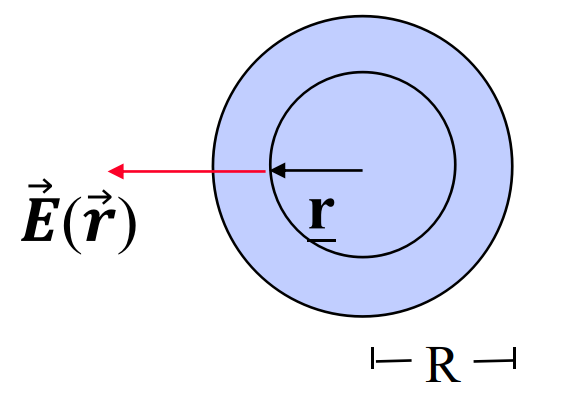
\includegraphics[width=130px]{28.png}
    \end{center}

    Berapa muatan yang terlingkupi?\\
    Bola kecil memiliki sebagian kecil dari total muatan. Berapa bagiannya? Yaitu diberikan oleh rasio volume sebagai berikut.

    \[ \Phi = EA = E(4\pi r^2) \]

    Lalu apabila $\displaystyle \Phi = \frac{Q_{enc}}{\epsilon_0}$\\
    maka
    \[ E = \frac{(r^3/R^3)Q}{4\pi\epsilon_0 r^2} \]

    \textcolor{blue}{ \textbf{Untuk $r<R$}  }

    \[ \vec E (\vec r) = \frac{Q}{4\pi \epsilon_0 R^3}r \hat r \]

    \begin{center}
        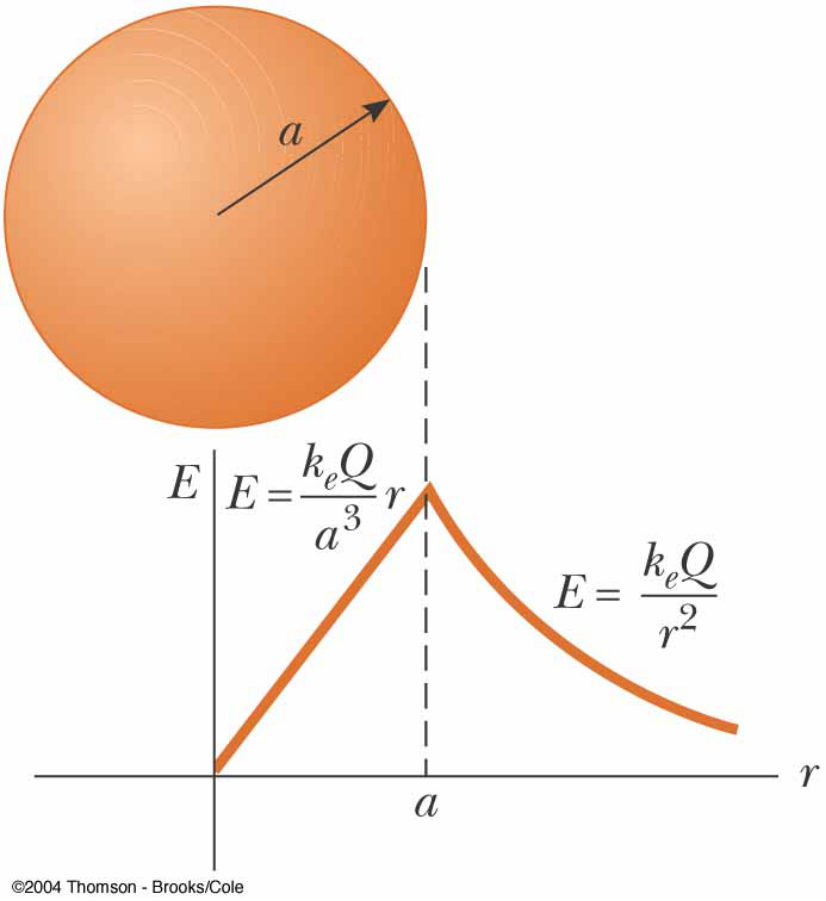
\includegraphics[width=200px]{29.png}
    \end{center}

    Sekarang perhatikan lebih dekat hasil ini. Medan listrik di \textcolor{red}{$\bullet$} berasal dari penjumlahan dari kontribusi semua bagian kecil $\color{blue}\blacksquare$.

    Jelas bahwa $\vec E$ pada titik ini akan horizontal. Tetapi besarnya dari setiap bagian kecil berbeda; dan itu sepenuhnya tidak jelas bahwa besaran E hanya bergantung pada jarak dari pusat bola ke titik observasi.

    \textbf{Melakukan ini sebagai integral volume akan menjadi SULIT.}\\
    \textbf{Hukum Gauss MUDAH.}
    
\end{document}
